\subsection{Statistical analysis of experiment 1}\label{subsec:Stat1}\todo{Split into expectations and result}

In this section the various statistical methods covered in \cref{subsec:correlation} and \cref{subsec:distribution} will be used to analyses the data. The initial step is to verify if the data is normally distributed as it has an effect on which statistical methods can be used to analyze the data. To do this the Shapiro-Wilk test will be used to check if the data is normally distributed. The results show that the data for the different DUTs are not all normally distributed, though the majority is.

\begin{table}[]
    \begin{tabular}{||c|c|c|c|c|c||}
    \hline
    &\textbf{TestCaseIdle}&\textbf{BinaryTrees}&\textbf{FannkuchRedux}&\textbf{Nbody}&\textbf{Fasta}\\ [0.5ex] \hline\hline
    \textbf{IntelPowerGadget}&0.0004&0.3685&0.0007&0.0&0.0809\\
    \textbf{HardwareMonitor}&0.0&0.0033&0.088&0.0&0.0002\\
    \textbf{E3}&0.9307&0.2229&0.0&0.0966&0.0002\\
    \textbf{RAPL}&0.0152&0.0311&0.0&0.0&0.0007\\ \hline
    \end{tabular}
    \label{tab:NormDistSurfB}
\end{table}

As can be seen in \cref{tab:NormDistSurfB}, the majority of the results are normally distributed given $P = 0.05$\todo{is 0.05 mentioned somewhere}. This is however not the case for all results, which is why the statistical methods able to handle non-normally distributed data is used. The first test is the MannWhitney U test, which is a non-parametric independence test, allowing a comparison of the different measurement foreach of the test cases to check if they are are independent from each other. The null hypothesis $H_0$ for the Mann-Whitney U test is defined as:

\begin{quote}
    \textit{In the population, the sum of the rankings in the two groups does not differ.}
\end{quote}

The expectation is that the $H_0$ can be rejected as each of the DUTs have different energy consumptions, and that each of the measuring instruments are different.
The results from the FannkuchRedux test case can be seen below, where the results for the remaining test cases can be found in the appendix.\todo{cref til dem}
\begin{figure}
  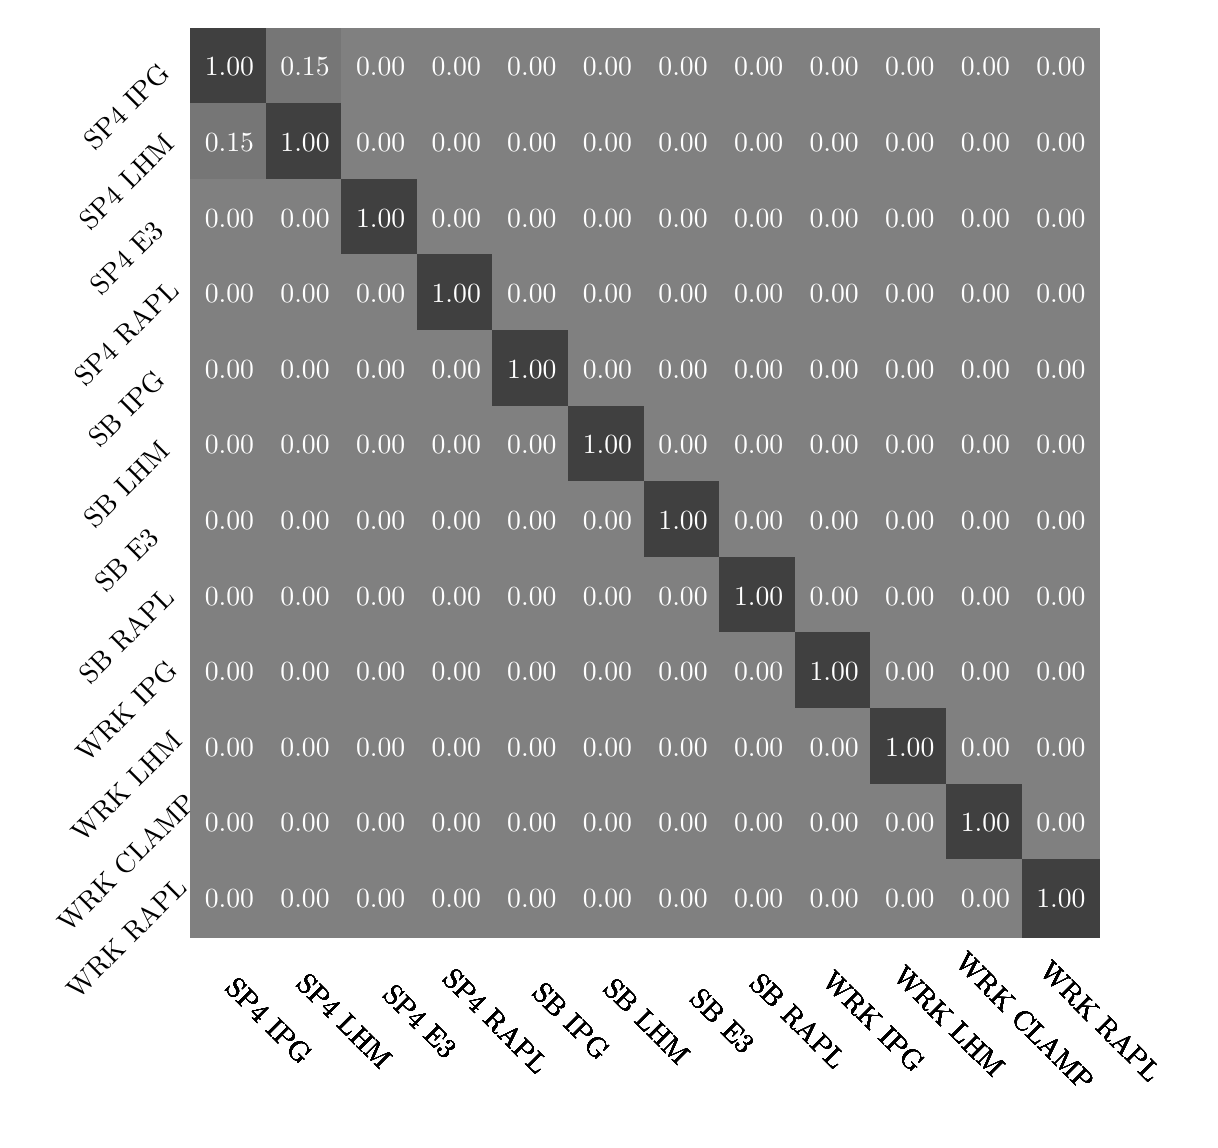
\begin{tikzpicture}[scale=0.6]
    \foreach \y [count=\n] in {{1.00, 0.15, 0.00, 0.00, 0.00, 0.00, 0.00, 0.00, 0.00, 0.00, 0.00, 0.00},{0.15, 1.00, 0.00, 0.00, 0.00, 0.00, 0.00, 0.00, 0.00, 0.00, 0.00, 0.00},{0.00, 0.00, 1.00, 0.00, 0.00, 0.00, 0.00, 0.00, 0.00, 0.00, 0.00, 0.00},{0.00, 0.00, 0.00, 1.00, 0.00, 0.00, 0.00, 0.00, 0.00, 0.00, 0.00, 0.00},{0.00, 0.00, 0.00, 0.00, 1.00, 0.00, 0.00, 0.00, 0.00, 0.00, 0.00, 0.00},{0.00, 0.00, 0.00, 0.00, 0.00, 1.00, 0.00, 0.00, 0.00, 0.00, 0.00, 0.00},{0.00, 0.00, 0.00, 0.00, 0.00, 0.00, 1.00, 0.00, 0.00, 0.00, 0.00, 0.00},{0.00, 0.00, 0.00, 0.00, 0.00, 0.00, 0.00, 1.00, 0.00, 0.00, 0.00, 0.00},{0.00, 0.00, 0.00, 0.00, 0.00, 0.00, 0.00, 0.00, 1.00, 0.00, 0.00, 0.00},{0.00, 0.00, 0.00, 0.00, 0.00, 0.00, 0.00, 0.00, 0.00, 1.00, 0.00, 0.00},{0.00, 0.00, 0.00, 0.00, 0.00, 0.00, 0.00, 0.00, 0.00, 0.00, 1.00, 0.00},{0.00, 0.00, 0.00, 0.00, 0.00, 0.00, 0.00, 0.00, 0.00, 0.00, 0.00, 1.00},} {
    % column labels
    \foreach \a [count=\n] in {SP4 IPG,SP4 LHM,SP4 E3,SP4 RAPL,SB IPG,SB LHM,SB E3,SB RAPL,WRK IPG,WRK LHM,WRK CLAMP,WRK RAPL} {
      \node[minimum size=10mm, xshift=0.5cm, rotate=-45] at (\n*1.6, -21.8) {\a};
    }
    % heatmap tiles
    \foreach \x [count=\m] in \y {
      \pgfmathsetmacro{\xa }{(\x + 1) / 2 * 100}
      \node[fill=darkgray!\xa!lightgray, minimum size=10mm, text=white, font={\normalsize}] at (\m*1.6,-\n*1.6) {\x};
    }
  }
    % row labels
    \foreach \a [count=\i] in {SP4 IPG,SP4 LHM,SP4 E3,SP4 RAPL,SB IPG,SB LHM,SB E3,SB RAPL,WRK IPG,WRK LHM,WRK CLAMP,WRK RAPL} {
      \node[minimum size=10mm, xshift=-0.35cm, yshift=-0.5cm, rotate=45] at (0,-\i*1.6) {\a};
    }
  \end{tikzpicture}
  \caption{Here the results for the FannkuchRedux can be seen}
  \label{tab:HeatFannkuchRedux}
  \end{figure} 

As can be seen in \cref{tab:HeatFannkuchRedux}, the majority of the values are below $p = 0.05$, meaning that we can confidently reject the null hypotheses. The only cases where $H_0$ cannot be rejected is SP4 LHM and SP4 IPG. This aligns with the expectations that the samples are independent of each other.

Following this, the correlation between the different measuring instruments will be compared using Kendall Tau correlation. When using the Kendall Tau Correlation, the test case results for each of the DUTs were appended to each other and sorted based on the test case, an example of which can be seen in \cref{tab:RainBowGraph}.

\input{tabels/experiment_results/exp_one/StatQuest/stats.tex}

In \cref{tab:RainBowGraph} the background represents which test case the data point is a measurement of and these are then used to calculate the correlation as seen in \cref{tab:correlationWork} and \cref{tab:HeatFasta}.

\begin{figure}
\centering
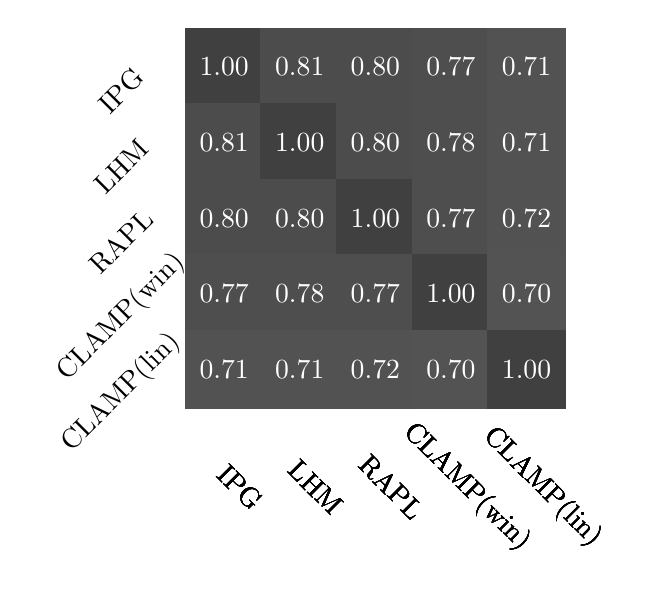
\begin{tikzpicture}[scale=0.6]
  \foreach \y [count=\n] in {{1.00, 0.81, 0.80, 0.77, 0.71},{0.81, 1.00, 0.80, 0.78, 0.71},{0.80, 0.80, 1.00, 0.77, 0.72},{0.77, 0.78, 0.77, 1.00, 0.70},{0.71, 0.71, 0.72, 0.70, 1.00},} {
  % column labels
  \foreach \a [count=\n] in {IPG,LHM,RAPL,CLAMP(win),CLAMP(lin)} {
    \node[minimum size=10mm, xshift=0.2cm, rotate=-45] at (\n*1.6, -10.50) {\a};
  }
  % heatmap tiles
  \foreach \x [count=\m] in \y {
    \pgfmathsetmacro{\xa }{(\x + 1) / 2 * 100}
    \node[fill=darkgray!\xa!lightgray, minimum size=10mm, text=white, font={\normalsize}] at (\m*1.6,-\n*1.6) {\x};
  }
}
  % row labels
  \foreach \a [count=\i] in {IPG,LHM,RAPL,CLAMP(win),CLAMP(lin)} {
    \node[minimum size=10mm, xshift=-0.35cm, yshift=-0.3cm, rotate=45] at (0,-\i*1.6) {\a};
  } 
\end{tikzpicture}
\caption{This heat map represents Correlation coefficients between the different measuring instruments -1 to 1 on the Workstation}
\label{tab:correlationWork}
\end{figure}
\begin{figure}
    \centering
    \begin{subfigure}{.5\textwidth}
      \centering
      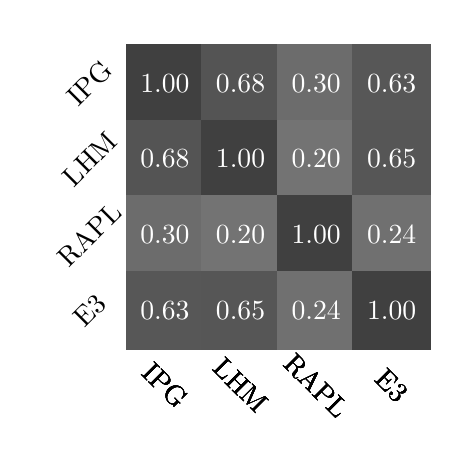
\begin{tikzpicture}[scale=0.6]
        \foreach \y [count=\n] in {{1.00, 0.68, 0.30, 0.63},{0.68, 1.00, 0.20, 0.65},{0.30, 0.20, 1.00, 0.24},{0.63, 0.65, 0.24, 1.00},} {
        % column labels
        \foreach \a [count=\n] in {IPG,LHM,RAPL,E3} {
          \node[minimum size=10mm, xshift=0.0cm, rotate=-45] at (\n*1.6, -8) {\a};
        }
        % heatmap tiles
        \foreach \x [count=\m] in \y {
          \pgfmathsetmacro{\xa }{(\x + 1) / 2 * 100}
          \node[fill=darkgray!\xa!lightgray, minimum size=10mm, text=white, font={\normalsize}] at (\m*1.6,-\n*1.6) {\x};
        }
      }
        % row labels
        \foreach \a [count=\i] in {IPG,LHM,RAPL,E3} {
          \node[minimum size=10mm, xshift=-0.0cm, yshift=-0.0cm, rotate=45] at (0,-\i*1.6) {\a};
        }
      \end{tikzpicture}
    \caption{This heat map represents Correlation coefficients between the different measurement instruments -1 to 1 on the Surface Book}
    \label{tab:correlationSurfP}
    \end{subfigure}%
    \begin{subfigure}{.5\textwidth}
      \centering
      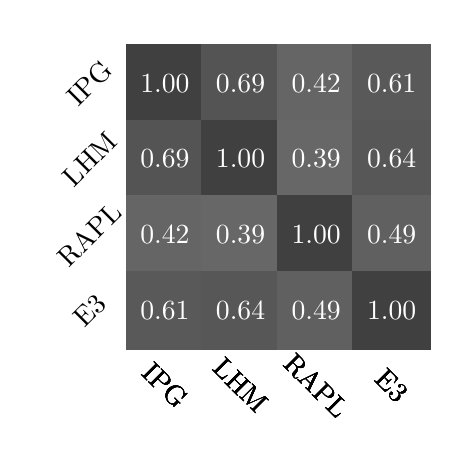
\begin{tikzpicture}[scale=0.6]
        \foreach \y [count=\n] in {{1.00, 0.69, 0.42, 0.61},{0.69, 1.00, 0.39, 0.64},{0.42, 0.39, 1.00, 0.49},{0.61, 0.64, 0.49, 1.00},} {
        % column labels
        \foreach \a [count=\n] in {IPG,LHM,RAPL,E3} {
          \node[minimum size=10mm, xshift=0.0cm, rotate=-45] at (\n*1.6, -8) {\a};
        }
        % heatmap tiles
        \foreach \x [count=\m] in \y {
          \pgfmathsetmacro{\xa }{(\x + 1) / 2 * 100}
          \node[fill=darkgray!\xa!lightgray, minimum size=10mm, text=white, font={\normalsize}] at (\m*1.6,-\n*1.6) {\x};
        }
      }
        % row labels
        \foreach \a [count=\i] in {IPG,LHM,RAPL,E3} {
          \node[minimum size=10mm, xshift=-0.0cm, yshift=-0.0cm, rotate=45] at (0,-\i*1.6) {\a};
        }
      \end{tikzpicture}
    \caption{This heat map represents Correlation coefficients between the different measurement instruments -1 to 1 on the Surface Pro 4}
    \label{tab:HeatFasta}
    \end{subfigure}
\end{figure}
% \begin{figure}
    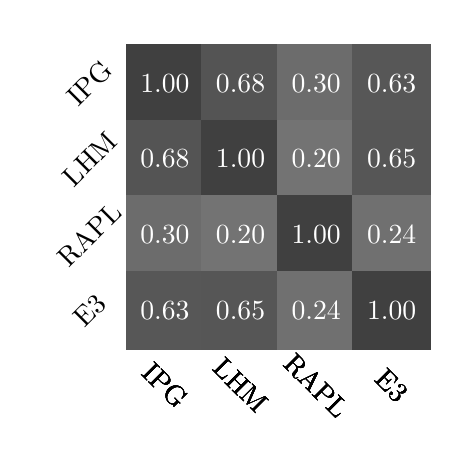
\begin{tikzpicture}[scale=0.6]
        \foreach \y [count=\n] in {{1.00, 0.68, 0.30, 0.63},{0.68, 1.00, 0.20, 0.65},{0.30, 0.20, 1.00, 0.24},{0.63, 0.65, 0.24, 1.00},} {
        % column labels
        \foreach \a [count=\n] in {IPG,LHM,RAPL,E3} {
          \node[minimum size=10mm, xshift=0.0cm, rotate=-45] at (\n*1.6, -8) {\a};
        }
        % heatmap tiles
        \foreach \x [count=\m] in \y {
          \pgfmathsetmacro{\xa }{(\x + 1) / 2 * 100}
          \node[fill=darkgray!\xa!lightgray, minimum size=10mm, text=white, font={\normalsize}] at (\m*1.6,-\n*1.6) {\x};
        }
      }
        % row labels
        \foreach \a [count=\i] in {IPG,LHM,RAPL,E3} {
          \node[minimum size=10mm, xshift=-0.0cm, yshift=-0.0cm, rotate=45] at (0,-\i*1.6) {\a};
        }
      \end{tikzpicture}
    \caption{This heat map represents Correlation coefficients between the different measurement instruments -1 to 1 on the Surface Book}
    \label{tab:correlationSurfP}
\end{figure}
% \begin{figure}
    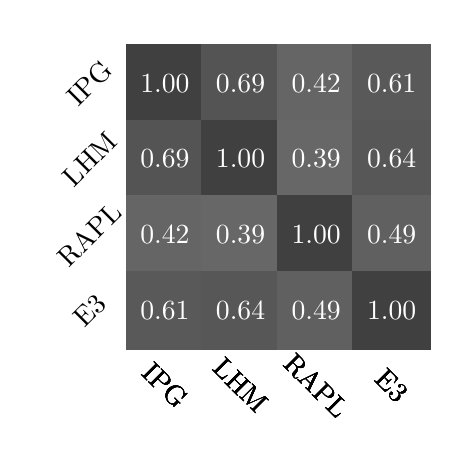
\begin{tikzpicture}[scale=0.6]
        \foreach \y [count=\n] in {{1.00, 0.69, 0.42, 0.61},{0.69, 1.00, 0.39, 0.64},{0.42, 0.39, 1.00, 0.49},{0.61, 0.64, 0.49, 1.00},} {
        % column labels
        \foreach \a [count=\n] in {IPG,LHM,RAPL,E3} {
          \node[minimum size=10mm, xshift=0.0cm, rotate=-45] at (\n*1.6, -8) {\a};
        }
        % heatmap tiles
        \foreach \x [count=\m] in \y {
          \pgfmathsetmacro{\xa }{(\x + 1) / 2 * 100}
          \node[fill=darkgray!\xa!lightgray, minimum size=10mm, text=white, font={\normalsize}] at (\m*1.6,-\n*1.6) {\x};
        }
      }
        % row labels
        \foreach \a [count=\i] in {IPG,LHM,RAPL,E3} {
          \node[minimum size=10mm, xshift=-0.0cm, yshift=-0.0cm, rotate=45] at (0,-\i*1.6) {\a};
        }
      \end{tikzpicture}
    \caption{This heat map represents Correlation coefficients between the different measuring instrument1 on the Surface Pro 4}
    \label{tab:HeatFasta}
\end{figure}

When evaluating the results, the scale presented by Guildford in \cite[219]{guilford1950fundamental} to evaluate correlation can be used.

\begin{itemize}
    \item $<.20$: Slight; almost negligible relationship
    \item $.20-.40$: Low correlation; definite but small relationship
    \item $.40-.70$: Moderate correlation; substantial relationship
    \item $.70-.90$: High Correlation; marked relationship
    \item $.90-1$: Very high correlation; very dependable relationship
\end{itemize}

Using this scale we can evaluate the correlation between the different measuring instruments. Looking across the different DUTs we can calculate average correlation between each of the measuring instruments. When comparing the correlation between the different measuring instruments across all DUTs, the correlation is as following:

$$IPG|LHM = (0.68+0.81+0.69)/3 = 0.726$$
$$IPG|RAPL = (0.30+0.42+0.80)/3 = 0.506$$
$$LHM|RAPL = (0.80+0.39+0.21)/3 = 0.466$$

Now, the average correlation between the different software measuring instruments against the clamp will be calculated. This is done for only the workstation, as the the clamp was only used on this DUT.

$$IPG|Clamp = (0.77+0.71)/2 = 0.74$$
$$LHM|Clamp = (0.78+0.71)/2 = 0.745$$
$$RAPL|Clamp = (0.77+0.72)/2 = 0.745$$

Similarly, the average correlation between the different measuring instruments from the DUTs with a battery can be calculated, to see how they are correlated with E3.

$$IPG|E3 = (0.63+0.61)/2 = 0.62$$
$$LHM|E3 = (0.65+0.64)/2 = 0.645$$
$$RAPL|E3 = (0.24+0.49)/2 = 0.365$$

Looking at these numbers and evaluating them on the Guildford scale, we can see that IPG|LHM, IPG|Clamp and RAPL|Clamp all are highly correlated and marked relationships, while LHM|RAPL, LHM|RAPL,IPG|E3 and LHM|E3 has a substantial relationships. The lowest correlation between the measurements was found with RAPL|E3 which are a low on correlation.

These results seem to indicate that all of the measuring instruments are correlated, which is expected as they measure the energy consumption of the same test cases, on the same DUT's. Another interesting thing to note here is that the correlation between the measurements on the workstation are higher as opposed to the two laptops as can be seen on \cref{tab:correlationWork,tab:CobineddCorrelation}. From this it can be seen that most of the measuring instruments are at least moderate correlated, except RAPL|E3.

%and this is especially true when looking at the workstation. %Another interesting observation is that all the measurements are less correlated on the laptops than the Workstation.




